\chap{温度场预测、边界表示与计算效率}

本章评价给定炉温序列下的300步温度场预测，考察递归展开、物理损失和边界表示对误差累积的影响。测试覆盖控制曲线、材料参数及边界时间结构的外推，采用相同测试信息下的边界表示对照和跨求解器数值参考，并报告单轨迹计算代价与固定几何三维结果。炉温序列由实验设定，评价范围为开环状态递推。

\sect{完整轨迹预测的模型选择}

一维 C45 温变物性数据集包含120条轨迹，其中训练、验证、ID测试和控制曲线OOD分别为70、15、15和20条。各组比较共享相同轨迹划分；归一化量由训练集确定，检查点依据验证集300步滚动RMSE选择。除单种子计时外，结果均报告种子42、7和123的均值与样本标准差。种子间标准差描述训练随机性，场景差异采用独立轨迹配对统计。

\subsect{递归展开与误差累积}

递归推演的输入温度场来自模型上一时刻的预测。展开长度比较设置 $K=1$ 与 $K=5$，两组共享70条训练轨迹、网络容量、物理权重 $10^{-3}$、批量大小、120轮训练和三个随机种子。表\ref{tab:unroll_ablation}同时列出一步误差与完整轨迹误差。

\begin{table}[H]
  \centering
  \caption{相同训练设置下的展开长度消融，均值$\pm$样本标准差}
  \label{tab:unroll_ablation}
  \small
  \begin{tabular}{ccccc}
    \toprule
    $K$ & \shortstack{验证滚动\\RMSE} & \shortstack{ID 滚动\\RMSE} & \shortstack{控制 OOD\\滚动 RMSE} & \shortstack{ID 一步\\RMSE} \\
    \midrule
    1 & $2.063\pm0.187$ & $2.196\pm0.005$ & $\mathbf{5.046\pm0.469}$ & $0.02862\pm0.00029$ \\
    5 & $\mathbf{2.035\pm0.244}$ & $\mathbf{2.103\pm0.123}$ & $5.589\pm0.789$ & $0.02848\pm0.00184$ \\
    \bottomrule
  \end{tabular}
\end{table}

两种设置的ID一步RMSE均约为 \SI{0.0285}{\degreeCelsius}，完整轨迹RMSE约为 \SI{2}{\degreeCelsius}，递归误差明显累积。$K=5$ 的验证和ID滚动RMSE均值分别比 $K=1$ 低 $1.3\%$ 和 $4.2\%$，控制OOD均值高 $10.8\%$。依据验证均值，本文选择 $K=5$；其收益限于当前验证和ID结果，控制曲线外推误差随展开长度增加而增大。

\subsect{物理约束强度与控制曲线外推}

在 $K=5$ 下，数据模型与物理约束模型仅改变损失中的物理权重，比较结果见表\ref{tab:weight_results}。控制OOD采用未见炉温曲线类型，评价留出控制过程中的响应误差；检查点仍由验证集选择。

\begin{table}[H]
  \centering
  \caption{不同物理权重的三随机种子结果，均值$\pm$样本标准差}
  \label{tab:weight_results}
  \small
  \begin{tabular}{ccccc}
    \toprule
    $\lambda_{\mathrm{phy}}$ & 验证 RMSE & ID RMSE & OOD RMSE & OOD 物理残差 \\
    \midrule
    0 & $2.282\pm0.109$ & $2.389\pm0.139$ & $5.994\pm0.430$ & $127.41\pm7.36$ \\
    $10^{-3}$ & $\mathbf{2.035\pm0.244}$ & $\mathbf{2.103\pm0.123}$ & $\mathbf{5.589\pm0.789}$ & $70.35\pm4.24$ \\
    $10^{-2}$ & $2.242\pm0.109$ & $2.739\pm0.107$ & $6.865\pm1.202$ & $\mathbf{60.29\pm10.42}$ \\
    \bottomrule
  \end{tabular}
\end{table}

$\lambda_{\mathrm{phy}}=10^{-3}$ 的验证RMSE均值最低，选为一维模型的正式权重。相对数据模型，其ID误差均值降低 $11.9\%$，控制OOD总体RMSE均值降低 $6.8\%$，OOD离散物理残差降低 $44.8\%$；其中升温后冷却轨迹的RMSE均值降低 $10.1\%$。权重增至 $10^{-2}$ 后，离散残差减小，温度场误差增加。两项指标随权重呈不同变化，模型选择以验证轨迹精度为依据。

配对统计采用每条控制OOD轨迹三个种子RMSE的平均值，差值定义为物理模型减去数据模型。20条轨迹中12条改善、8条变差，平均配对差为 \SI{-0.220}{\degreeCelsius}；以轨迹为单位进行100000次bootstrap，95\%区间为 $[-0.588,0.153]$~\si{\degreeCelsius}。区间包含零，$6.8\%$ 的总体均值降幅仅构成当前样本中的改善趋势，稳定的控制OOD精度收益缺乏统计支持。各物理权重的重复结果见图\ref{fig:weight_results}。

\begin{figure}[H]
  \centering
  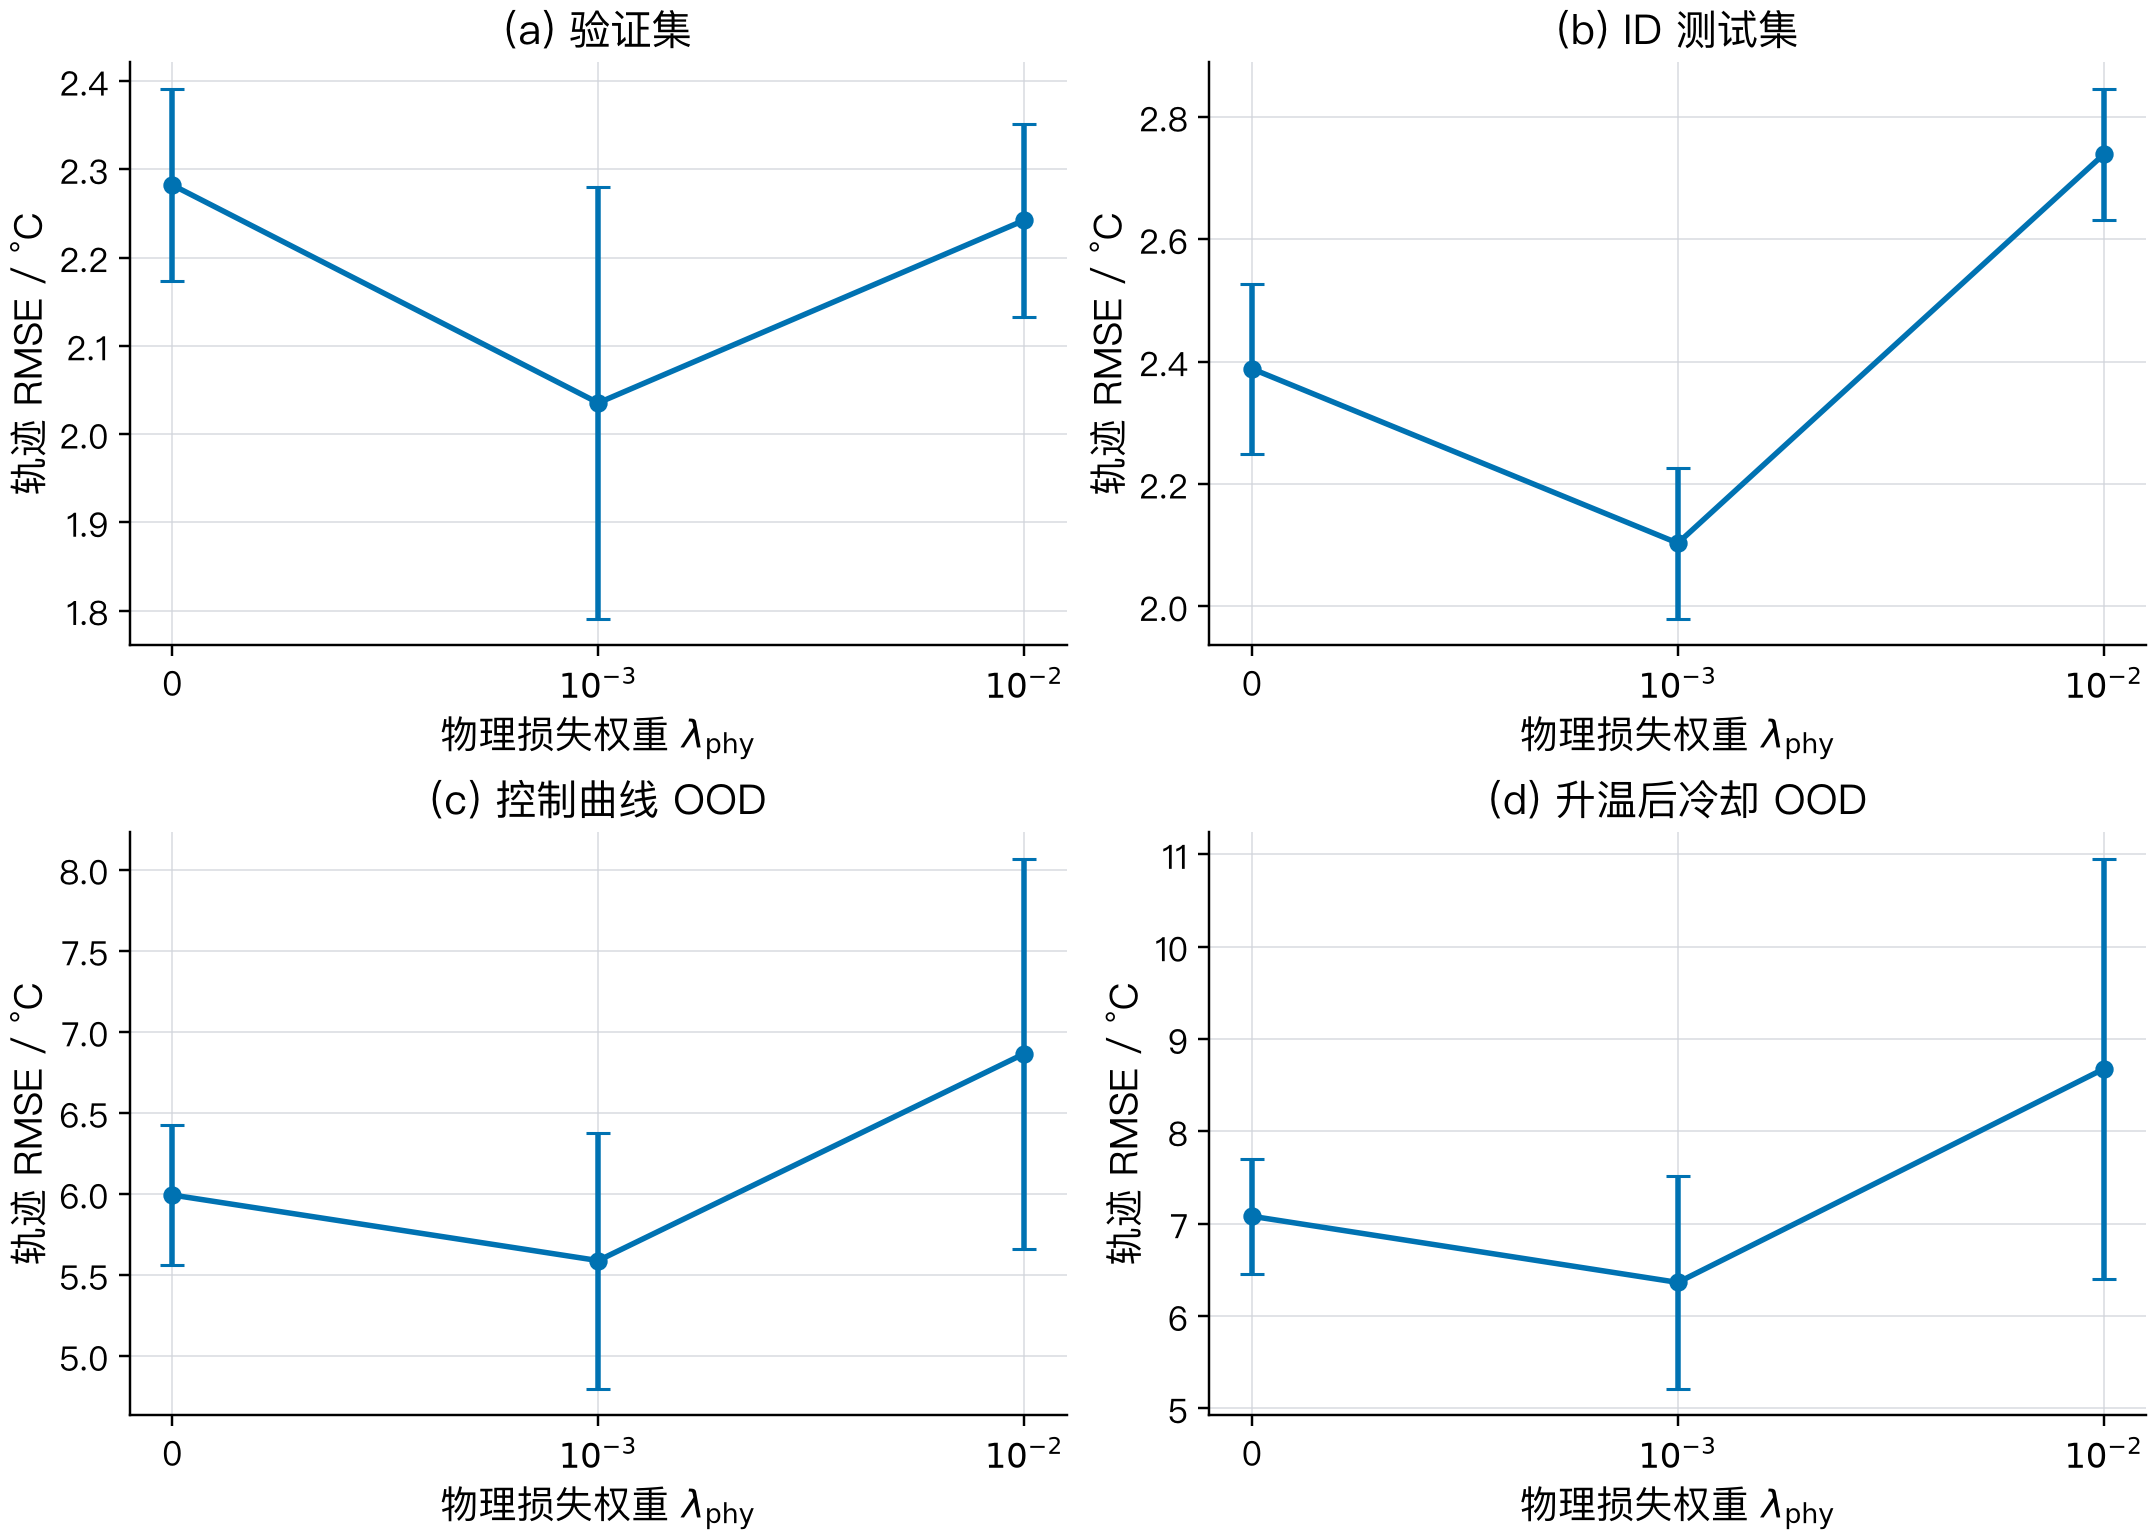
\includegraphics[width=0.96\textwidth]{physics_weight_replicates.png}
  \caption{物理权重在 ID 与控制 OOD 条件下的重复实验结果}
  \label{fig:weight_results}
\end{figure}

\sect{参数外推与边界时间结构}

\subsect{材料及边界参数范围的外推}

参数OOD集的控制曲线保持为训练类型，对流换热系数、发射率、导热系数尺度和比热尺度各设置20条单因素轨迹，另设置20条四参数组合轨迹，共100条。表\ref{tab:param_ood}比较数据模型与正式物理权重下的三种子结果。

\begin{table}[H]
  \centering
  \caption{参数 OOD 的滚动 RMSE，单位：\si{\degreeCelsius}}
  \label{tab:param_ood}
  \begin{tabular}{lccc}
    \toprule
    OOD 类型 & 数据模型 & 物理模型 & 相对降低 \\
    \midrule
    对流换热系数 $h$ & $3.082\pm0.259$ & $2.693\pm0.613$ & $12.6\%$ \\
    发射率 $\varepsilon$ & $3.239\pm0.290$ & $3.046\pm0.507$ & $6.0\%$ \\
    导热系数尺度 $s_k$ & $7.369\pm0.702$ & $5.633\pm0.397$ & $23.6\%$ \\
    比热尺度 $s_c$ & $5.802\pm0.445$ & $5.672\pm0.953$ & $2.2\%$ \\
    四参数组合 & $16.991\pm2.893$ & $11.972\pm2.534$ & $29.5\%$ \\
    \bottomrule
  \end{tabular}
\end{table}

五类参数OOD的平均RMSE均有所降低，其中导热系数尺度和四参数组合在三个种子下都得到改善。四参数组合的滚动RMSE由 $16.991\pm2.893$ 降至 $11.972\pm2.534$~\si{\degreeCelsius}，降幅为 $29.5\%$；最大绝对误差由 $121.76\pm30.94$ 降至 $61.69\pm16.41$~\si{\degreeCelsius}，离散物理残差由 $614.78\pm45.47$ 降至 $233.62\pm27.30$~\si{\degreeCelsius}。多参数偏移同时改变热扩散时间尺度和表面热流，组合工况在本组参数测试中的平均误差降幅最大。这些误差降幅仅适用于所测试的参数分布。

\begin{figure}[H]
  \centering
  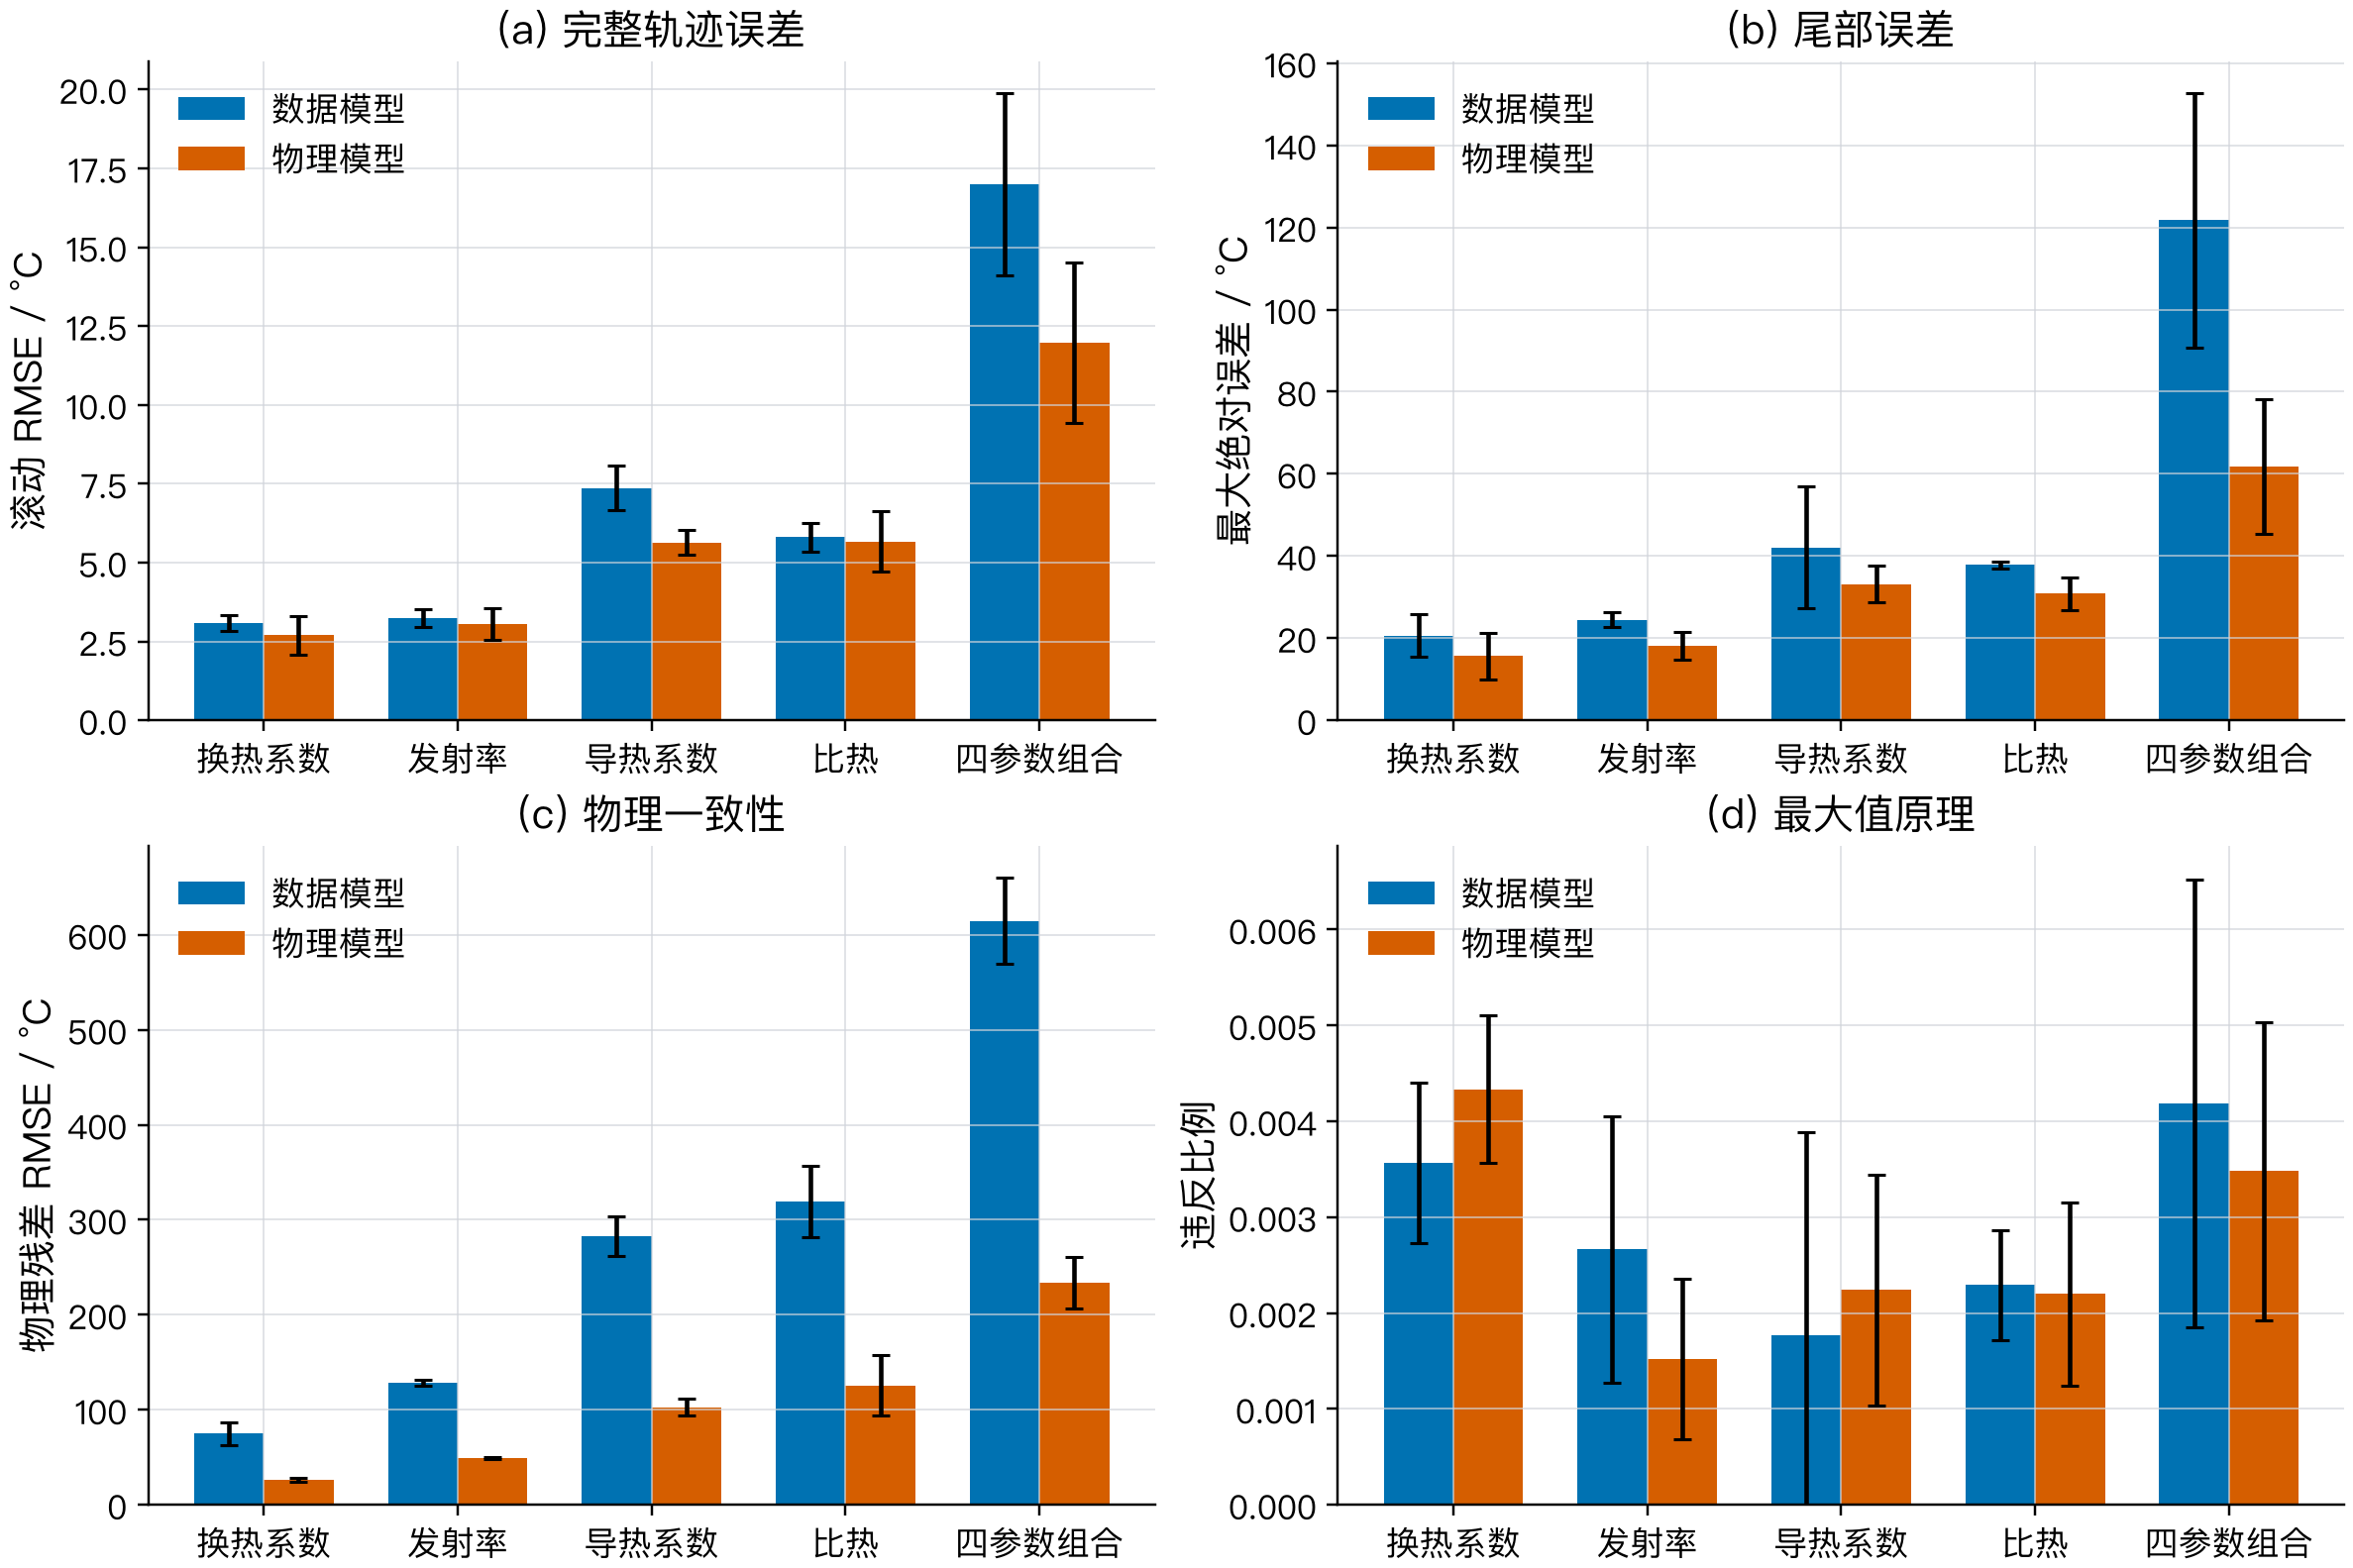
\includegraphics[width=0.96\textwidth]{parameter_ood_metrics.png}
  \caption{不同参数 OOD 类别的温度场推演误差}
  \label{fig:param_ood}
\end{figure}

\subsect{时变边界与逐步输入}

动态边界实验将参数值限制在训练范围内，只改变其时间结构。测试包含 $h$ 平滑变化、$h$ 阶跃、$\varepsilon$ 增长、$\varepsilon$ 阶跃和联合变化五类，共100条轨迹；训练轨迹中的边界参数在单条轨迹内保持常数。该设计评价训练参数范围内的时间结构外推。

逐步提供真实 $h(t)$ 和 $\varepsilon(t)$ 时，数据模型滚动RMSE为 $4.795\pm0.289$~\si{\degreeCelsius}，物理模型为 $4.089\pm0.162$~\si{\degreeCelsius}，均值降低 $14.7\%$；物理残差降低 $57.3\%$，逐轨迹RMSE的95\%分位数降低 $13.0\%$。整段推演固定使用首时刻参数时，两类模型的RMSE均约为 \SI{19.4}{\degreeCelsius}。固定边界引起的误差增幅大于两种损失设置之间的差异，两类模型均依赖逐步更新的边界信息。

图\ref{fig:dynamic_trajectory}取联合边界变化类别中的中位误差轨迹。在300~s内对流与辐射条件连续变化，模型接收逐步更新的真实边界值；物理模型在中心和表面位置均跟踪数值参考。该例评价真实时变边界已知条件下的预测，边界表示对照与未知边界估计分别在后续实验中处理。

\begin{figure}[H]
  \centering
  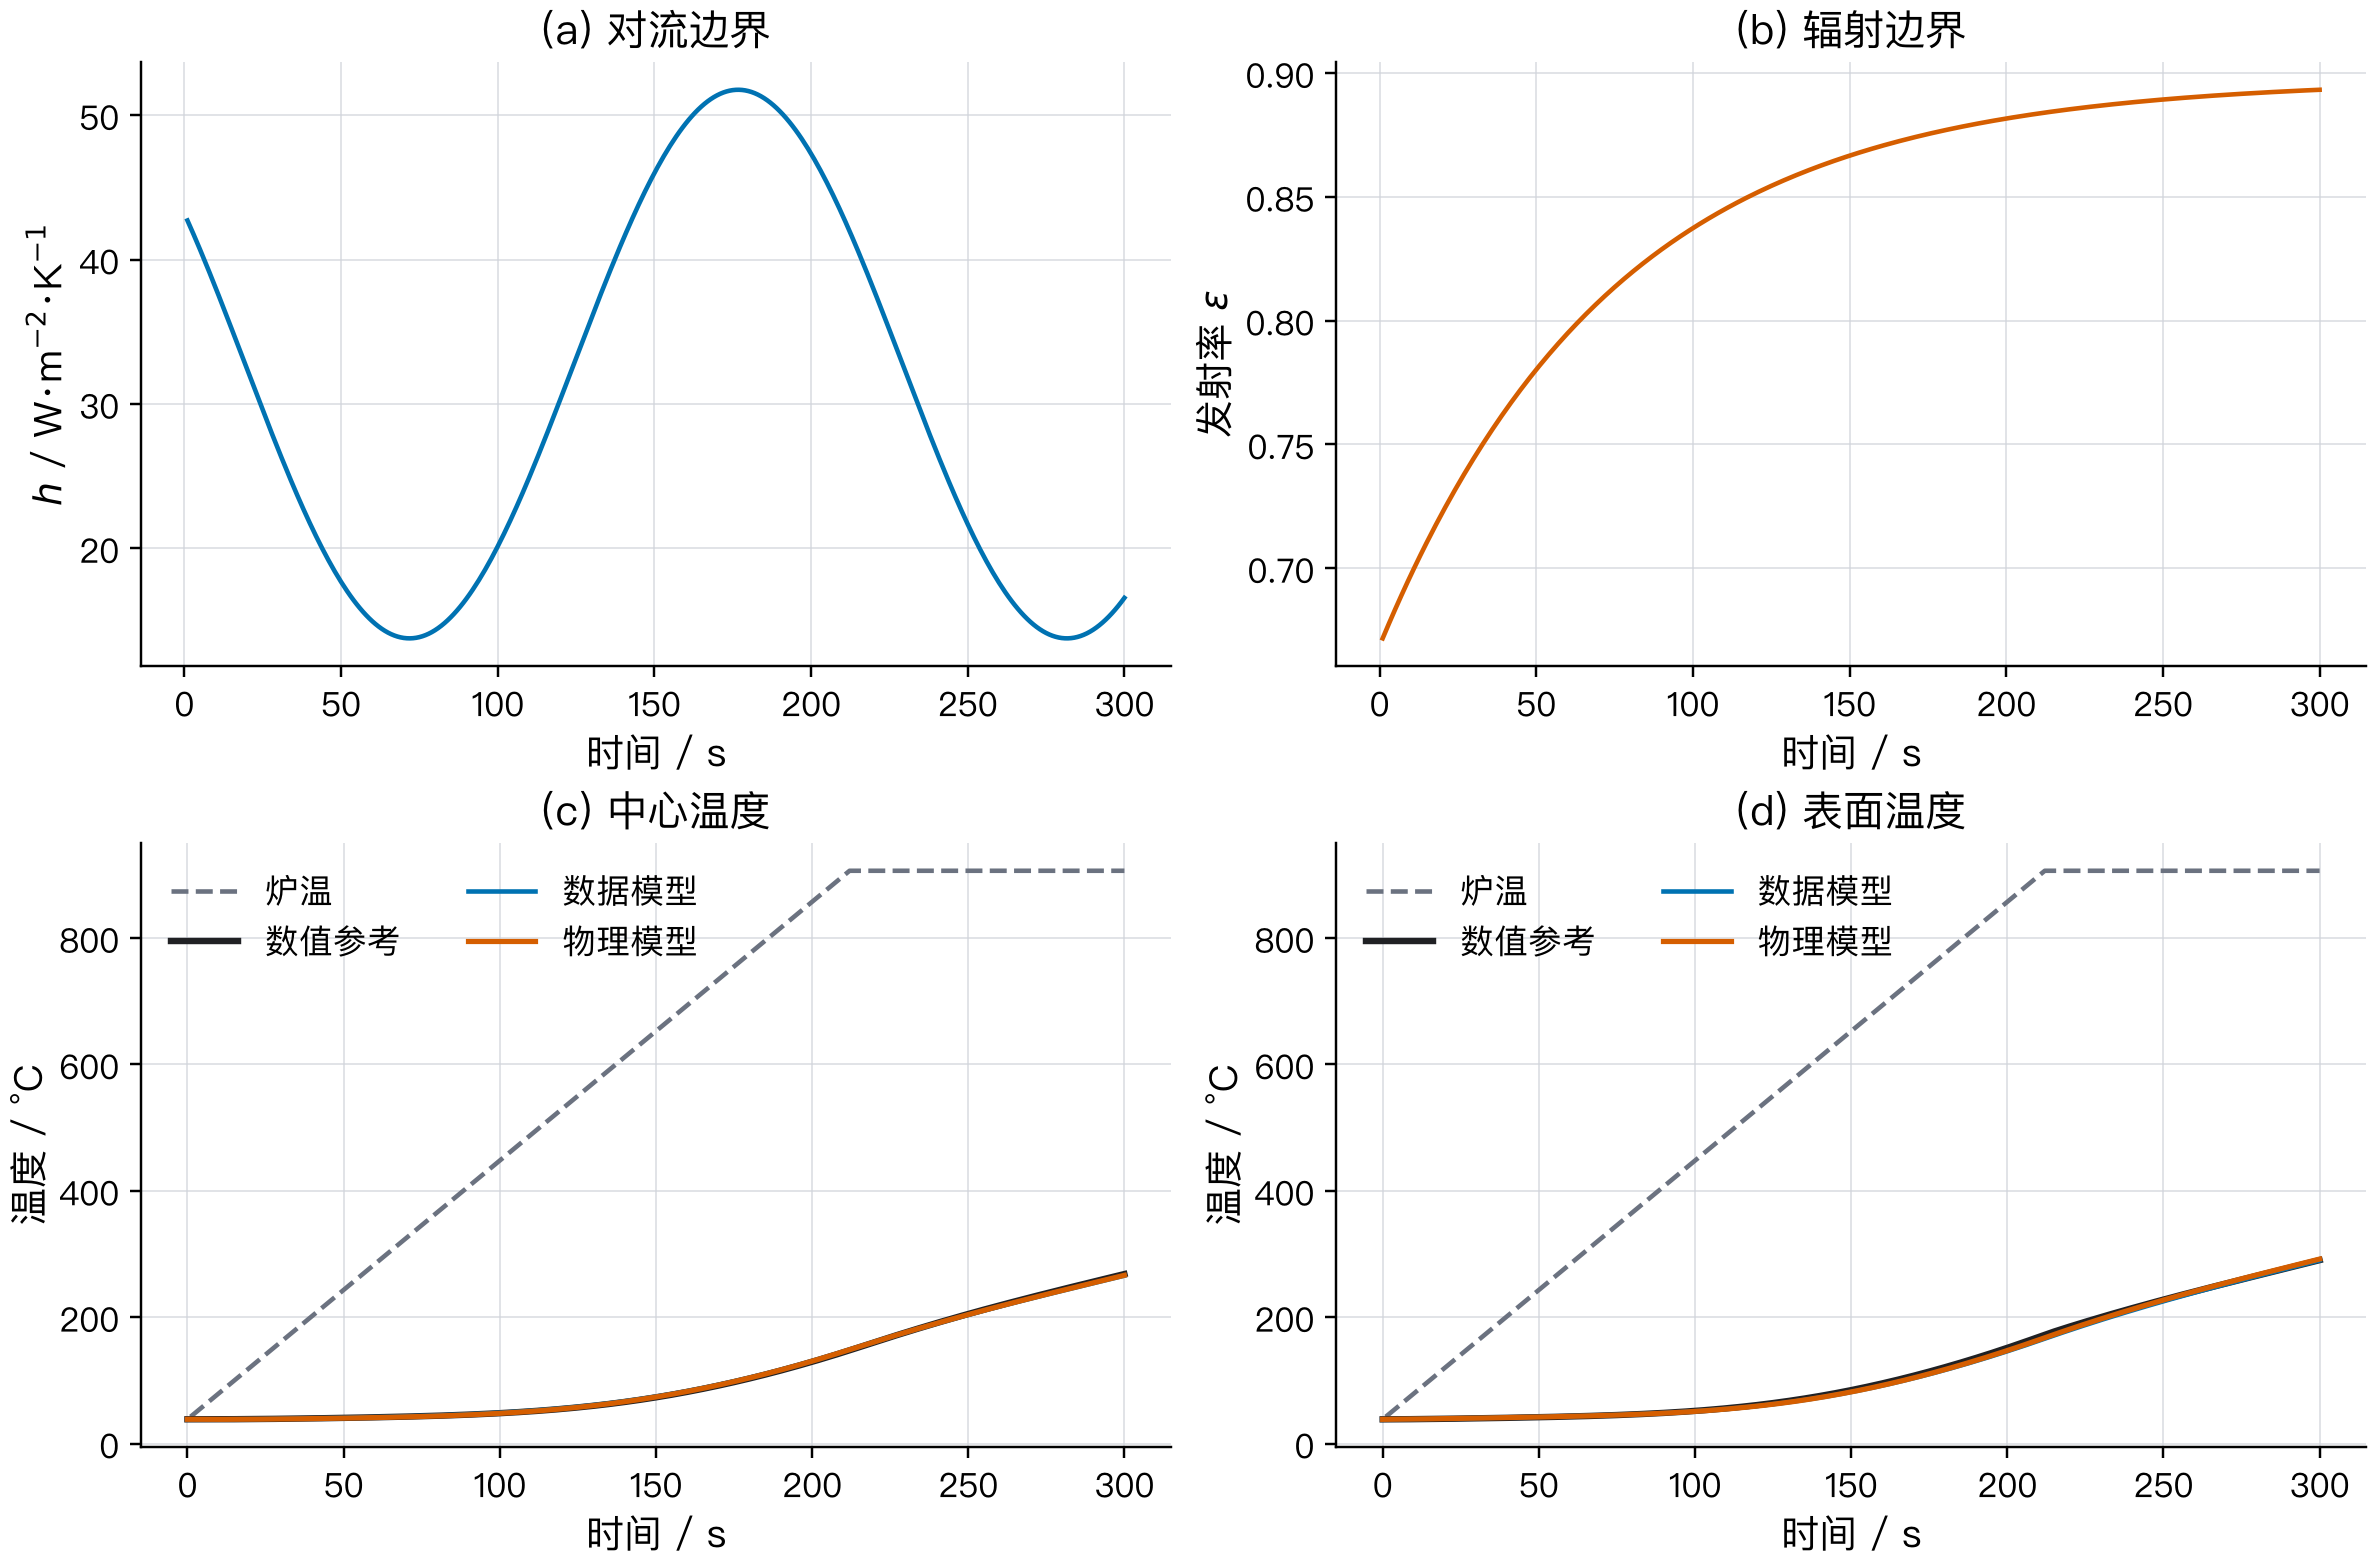
\includegraphics[width=0.96\textwidth]{dynamic_boundary_trajectory_zh.png}
  \caption{联合动态边界下的代表性温度场推演轨迹}
  \label{fig:dynamic_trajectory}
\end{figure}

\sect{等效边界表示与测试信息条件}

式\eqref{eq:heff}将当前对流与辐射热流写为等效换热系数 $\Heff$ 与边界温差的乘积。边界表示实验分别评价预测状态重算和参考状态条件输入。参考状态条件输入包含额外的表面温度信息，与直接接收 $h,\varepsilon$ 的自主模型具有不同的测试信息条件。

等效边界模型使用同一组120条静态边界轨迹，将每个转移的输入转换为 $\Heff$，保持训练、验证与测试划分、网络宽度和深度、训练轮数、随机种子及物理损失权重一致。多步训练和验证检查点选择采用由参考状态构造的 $\Heff$ 序列：温度场按网络输出递归，系数始终取自参考状态。自主滚动评价固定这些模型权重和检查点，未利用测试结果重新训练或选模。“自主”限定于测试推理阶段的系数更新，训练与验证仍采用参考状态条件输入。

测试使用另一组动态边界留出轨迹，同样包含五类边界变化、每类20条，共100条，每条递推300步。它与上一节动态边界测试属于不同抽样，误差不作跨数据集的直接差值比较。两种自主模型均获得相同的初始温度场、炉温序列、真实动态 $h,\varepsilon$ 和材料几何参数。原始参数模型直接使用 $h,\varepsilon$；等效边界模型在每一步取自身两端预测表面温度的平均值，代入式\eqref{eq:heff}重算 $\Heff$，不读取后续参考温度。参考表面温度条件输入作为单独的诊断对照列出。表\ref{tab:heff_results}中的模型物理权重均为 $10^{-3}$，离散残差统一使用真实 $h,\varepsilon$ 和各自预测状态计算。

\begin{table}[H]
  \centering
  \caption{动态边界留出集上的边界表示比较：三种子均值$\pm$样本标准差}
  \label{tab:heff_results}
  \begin{tabular}{lcc}
    \toprule
    边界输入与测试方式 & 滚动 RMSE/\si{\degreeCelsius} & 物理残差/\si{\degreeCelsius} \\
    \midrule
    $h,\varepsilon$，真实动态值 & $2.285\pm0.108$ & $17.79\pm1.59$ \\
    $\Heff$，由预测表面温度重算 & $1.494\pm0.082$ & $17.37\pm2.79$ \\
    $\Heff$，参考表面温度条件输入 & $1.409\pm0.068$ & $17.38\pm2.81$ \\
    \bottomrule
  \end{tabular}
\end{table}

相同测试信息下，滚动RMSE由 $2.285\pm0.108$ 降至 $1.494\pm0.082$~\si{\degreeCelsius}，均值降低 $34.6\%$。配对统计使用各轨迹三个种子RMSE的平均值，对100条轨迹进行100000次bootstrap，等效边界模型减去原始参数模型的配对差均值为 \SI{-0.459}{\degreeCelsius}，95\%区间为 $[-0.638,-0.305]$~\si{\degreeCelsius}，82/100条轨迹改善。该配对差基于逐轨迹RMSE的均值，与表中全场总体RMSE均值之差具有不同的汇总次序。

参考状态条件输入的误差为 $1.409\pm0.068$~\si{\degreeCelsius}，相对原始参数模型降低 $38.3\%$，其中包含额外状态信息的影响。自主预测对应的同信息降幅为 $34.6\%$。这组比较支持已知动态参数序列下、采用参考状态系数训练和验证的等效边界模型；完全自主系数训练与未知边界辨识均未在该对照中检验。未知边界的因果观测与状态估计见下一章。

\sect{跨求解器验证与计算代价}

\subsect{改变参考离散后的预测误差}

一维模型的训练数据与物理损失采用同一固定时间步长离散系统。跨求解器测试对边界表示留出集的相同100条物理工况，采用81节点空间离散和 SciPy 自适应BDF时间积分求解，并将参考场投影到模型网格。BDF轨迹仅用于评价，不参与网络训练与检查点选择。表\ref{tab:cross_solver}同时列出两种边界表示的数据模型与物理模型结果。

\begin{table}[H]
  \centering
  \caption{BDF 参考轨迹上的跨求解器数值验证}
  \label{tab:cross_solver}
  \begin{tabular}{lcc}
    \toprule
    模型 & 滚动 RMSE/\si{\degreeCelsius} & 最大绝对误差/\si{\degreeCelsius} \\
    \midrule
    $h,\varepsilon$ 数据模型 & $2.539\pm0.018$ & $25.56\pm0.43$ \\
    $h,\varepsilon$ 物理模型 & $2.316\pm0.092$ & $21.87\pm2.71$ \\
    $\Heff$ 数据模型，自主重算 & $1.551\pm0.050$ & $14.33\pm4.46$ \\
    $\Heff$ 物理模型，自主重算 & $1.560\pm0.092$ & $11.78\pm0.74$ \\
    $\Heff$ 数据模型，参考状态条件输入 & $1.491\pm0.065$ & $14.27\pm4.05$ \\
    $\Heff$ 物理模型，参考状态条件输入 & $1.460\pm0.078$ & $9.75\pm0.20$ \\
    \bottomrule
  \end{tabular}
\end{table}

在相同测试信息下，自主 $\Heff$ 物理模型相对 $h,\varepsilon$ 物理模型的总体RMSE均值降低 $32.6\%$，最大绝对误差均值降低 $46.1\%$。采用与前节相同的轨迹配对和100000次bootstrap方法，RMSE配对差均值为 \SI{-0.415}{\degreeCelsius}，95\%区间为 $[-0.598,-0.260]$~\si{\degreeCelsius}，80/100条轨迹改善。图\ref{fig:cross_solver_summary}将两套数值参考上的结果并列，等效边界模型的预测改善在BDF参考上仍然存在。

同一种自主 $\Heff$ 表示下，物理模型的总体RMSE为 \SI{1.560}{\degreeCelsius}，高于数据模型的 \SI{1.551}{\degreeCelsius}，最大绝对误差则较低。参考状态条件结果包含额外温度信息；所有 $\Heff$ 模型的训练与验证条件均保持前节设置。两套参考共用100条物理工况，按200个独立场景合并统计会重复计数。跨求解器结果评价数值实现变化下的预测表现，真实炉体验证仍待开展。

\begin{figure}[H]
  \centering
  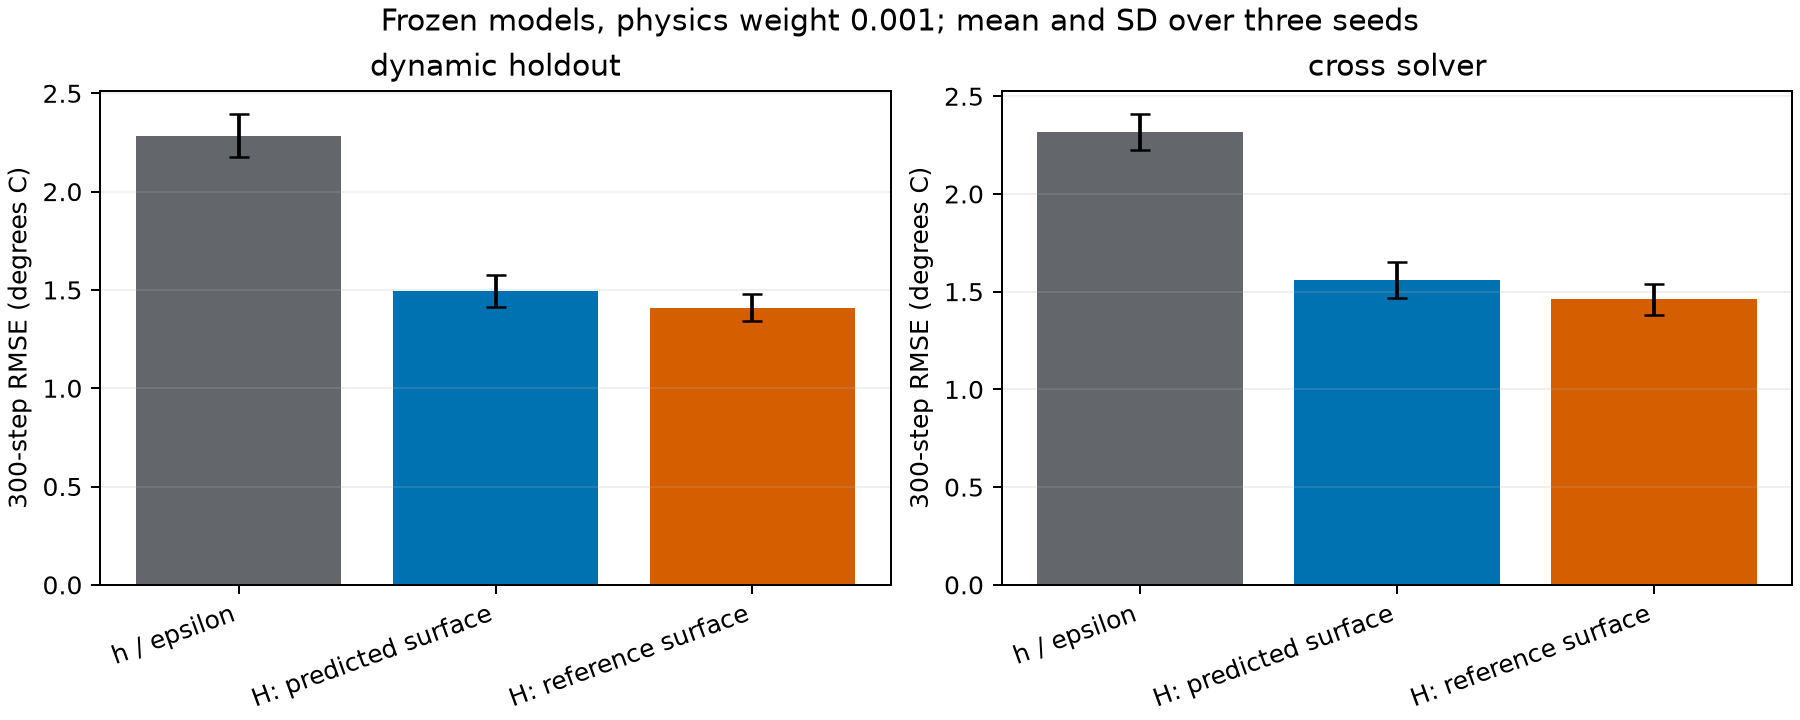
\includegraphics[width=0.98\textwidth]{fair_boundary_comparison.png}
  \caption{同信息自主滚动与参考表面温度条件输入的比较，误差棒表示三个训练种子的样本标准差}
  \label{fig:cross_solver_summary}
\end{figure}

图\ref{fig:cross_solver_trajectory}采用联合边界类别中、两种数值求解器差异最接近类别中位数的轨迹。固定步长数值解与BDF解在该例中接近。图内 $\Heff$ 曲线使用参考状态构造系数，展示条件输入下的时间响应；自主重算精度由表\ref{tab:cross_solver}单独报告。

\begin{figure}[H]
  \centering
  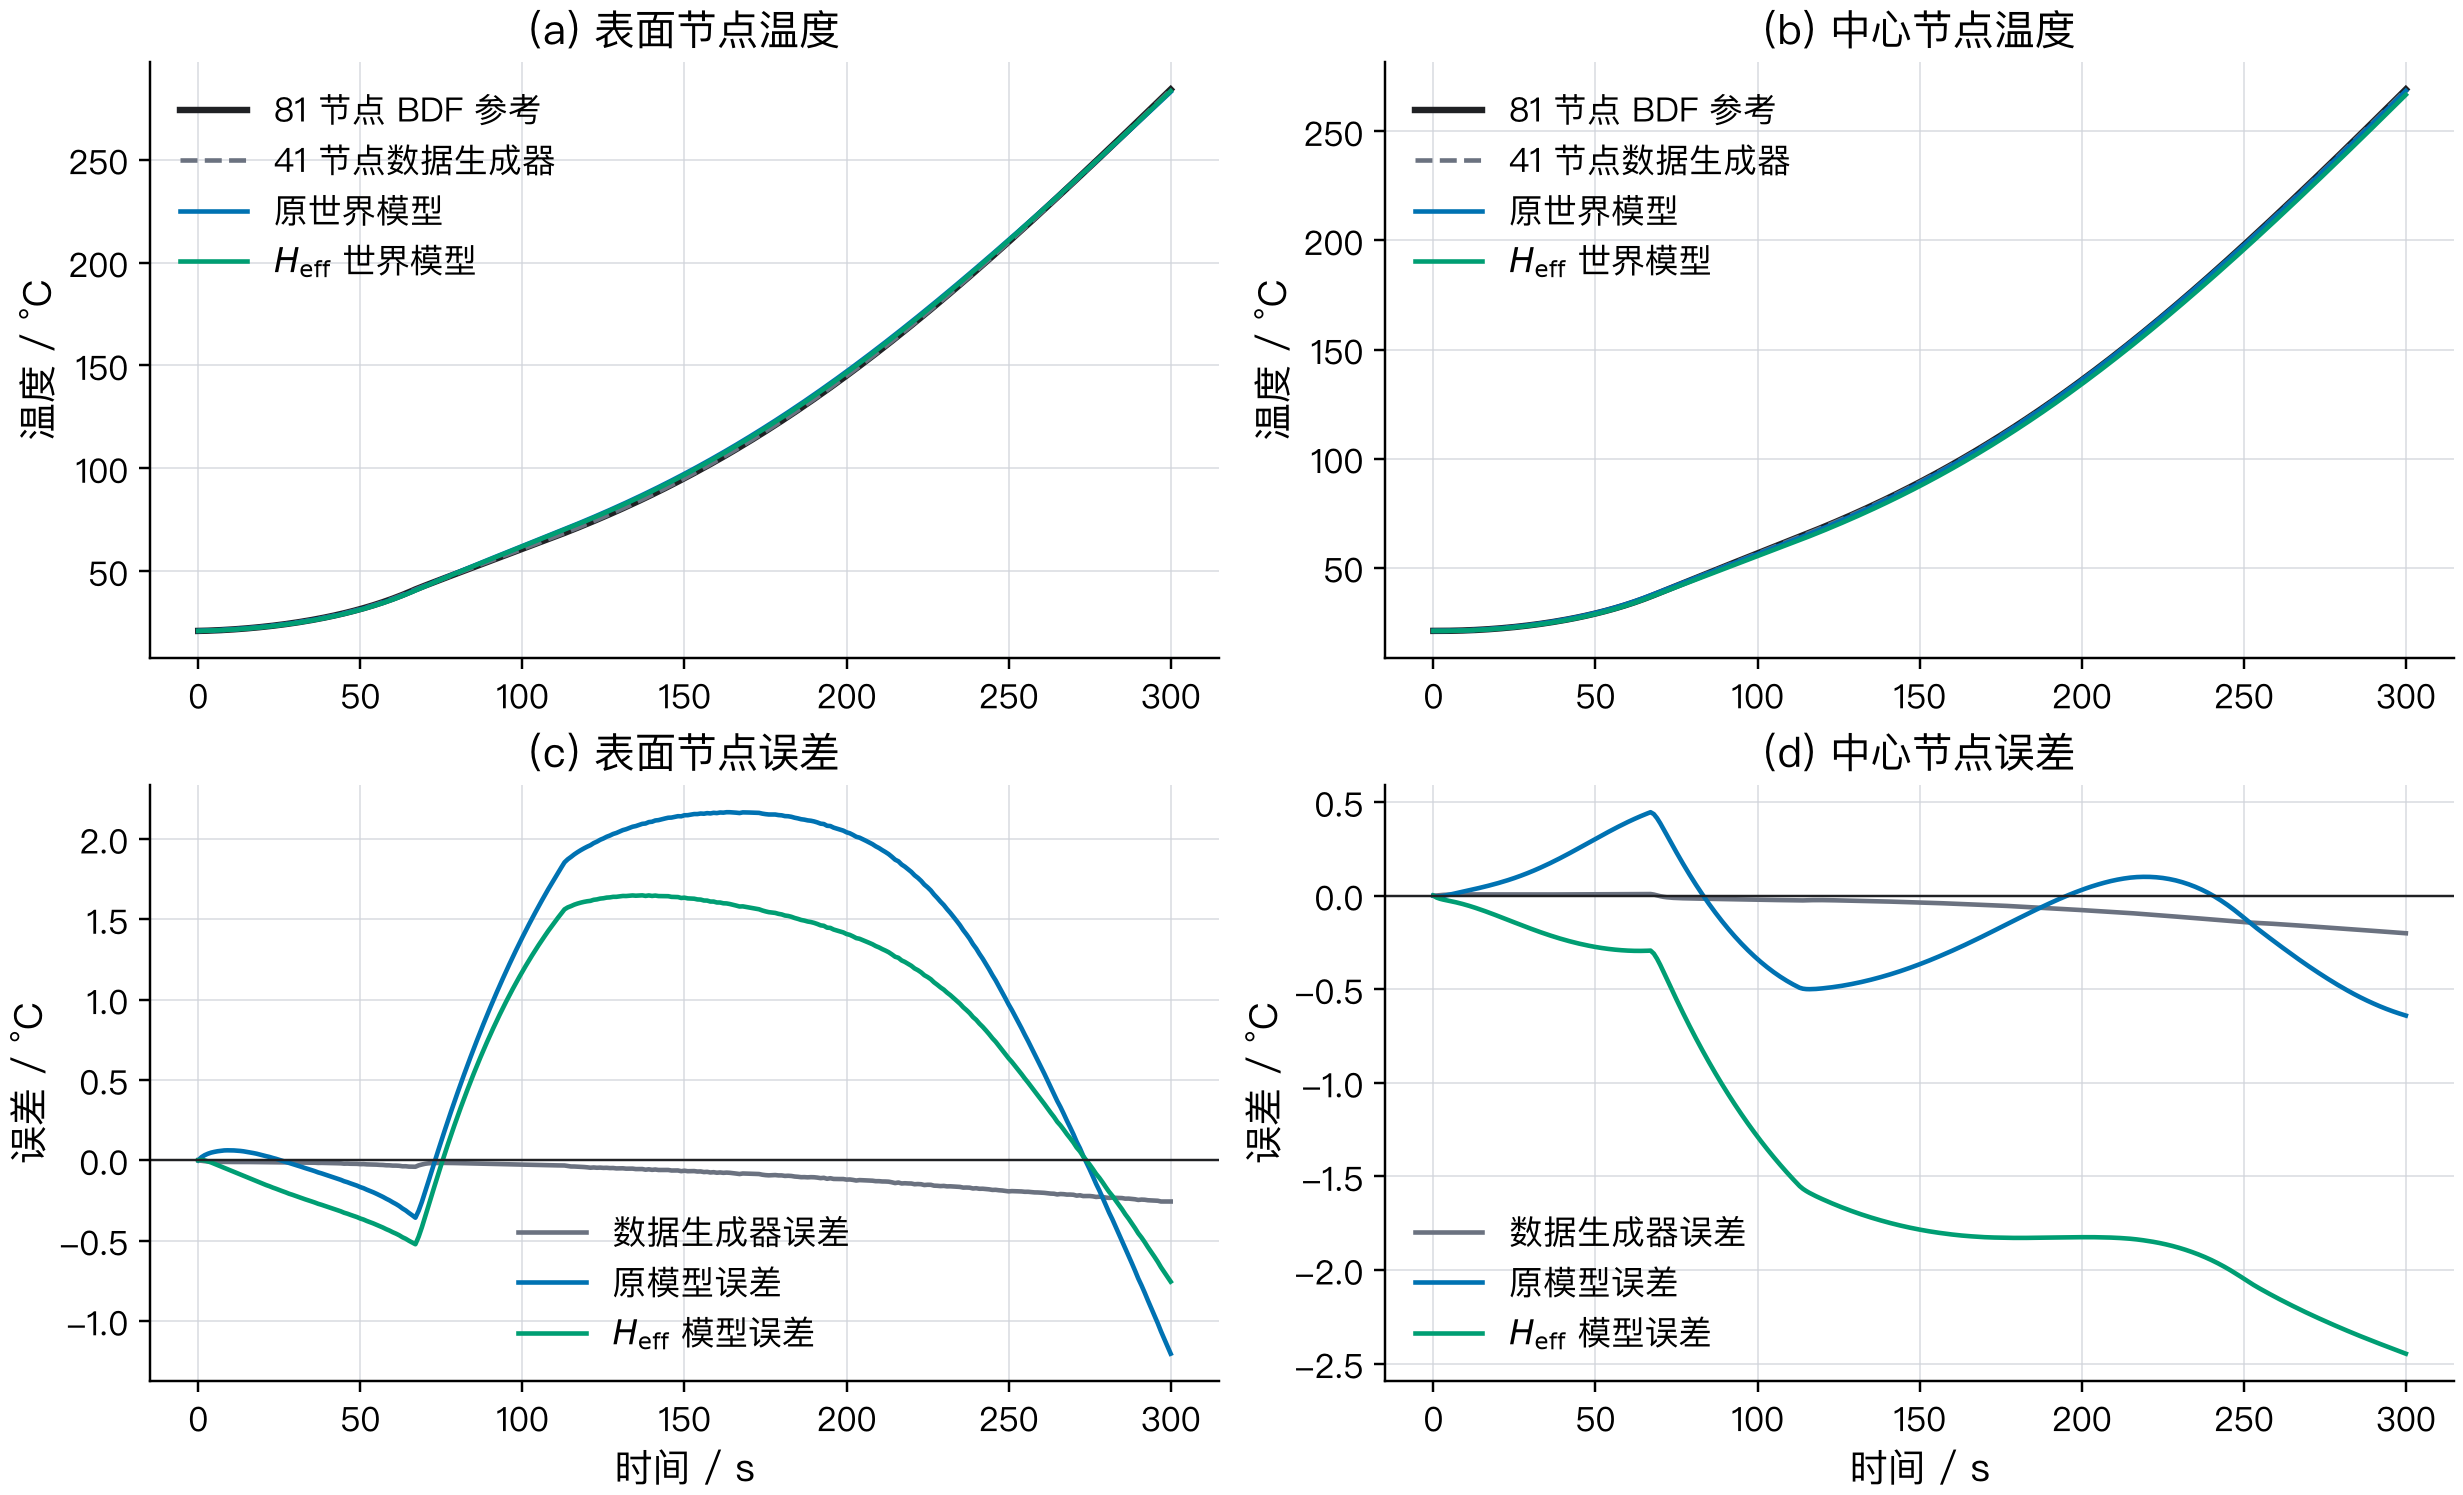
\includegraphics[width=0.96\textwidth]{cross_solver_trajectory_zh.png}
  \caption{代表性动态边界轨迹的跨求解器温度曲线（有效边界采用参考状态条件输入）}
  \label{fig:cross_solver_trajectory}
\end{figure}

\subsect{相同工作量下的单轨迹计算代价}

计时比较在 Apple M5 CPU 上以单线程运行，使用上述相同100条输入轨迹，每条包含300步转移。神经模型固定为种子42、物理权重0.001，比较原始 $h,\varepsilon$ 网络、自主 $\Heff$ 网络、41节点固定步长数值模型和81节点BDF。BDF相对与绝对容差分别为 $10^{-6}$ 和 $10^{-7}$，最大步长为 \SI{0.25}{\second}。

四种方法均预热一整轮，正式计时三整轮，每条场景内随机排列方法顺序；每种方法的300次计时来自100条不同工况。计时包含输入转换、自主 $\Heff$ 更新、输出数组形成及BDF投影，模型载入与求解器构造均不计入，运行期间暂停其他实验计算。表\ref{tab:fair_timing}同时给出耗时和相对缓存BDF参考解的误差，精度指标对应单个种子，与三种子结果分别报告。

\begin{table}[H]
  \centering
  \caption{相同 100 条场景完整推演的耗时与精度（每种方法 300 次计时）}
  \label{tab:fair_timing}
  \begin{tabular}{lrrr}
    \toprule
    方法 & 中位耗时/ms & 95 分位/ms & RMSE/\si{\degreeCelsius} \\
    \midrule
    原始 $h,\varepsilon$ 网络 & 8.116 & 8.607 & 2.345 \\
    自主 $\Heff$ 网络 & 10.284 & 10.962 & 1.474 \\
    41 节点固定步长数值模型 & 10.873 & 11.351 & 0.166 \\
    81 节点 BDF & 452.847 & 562.346 & $4.1\times10^{-6}$ \\
    \bottomrule
  \end{tabular}
\end{table}

81节点BDF的中位耗时是自主 $\Heff$ 网络的44.0倍；41节点固定步长数值模型的中位耗时为该网络的1.06倍，RMSE更低。比较固定了实现和离散配置，未匹配数值方法与网络的预测精度。网络相对于BDF复核器具有计算余量，相对于简单数值模型的一维单轨迹精度与效率综合优势尚未确立。

下一章的63.4倍规划耗时比对应完整状态及未来边界已知条件下的候选动作搜索，本节的44.0倍对应一次完整轨迹预测，两者的工作量与信息条件不同。候选动作批量推演的同精度数值基准、优化降阶模型对照及三维闭环计时仍未完成，速度结论限于所报告的任务和基准。

\sect{三维温度场的递推与误差结构}

\subsect{固定几何下的训练与评价协议}

三维实验评价固定几何下较多温度状态的受控递推。三维热模型可用于表达氧化层、支承遮蔽和各表面非均匀受热的影响\cite{yang2022reheating3d}；本节采用均匀六面边界，不包含这些复杂表面条件。C45试块尺寸为 \SI{60}{\milli\metre}$\times$\SI{40}{\milli\metre}$\times$\SI{20}{\milli\metre}，材料物性和对流--辐射边界与一维模型一致。

基础网格为 $9\times7\times5$，含315个温度状态；加密网格为 $17\times13\times9$，含1989个状态。两套网格均用方法线与BDF生成参考轨迹，每条包含300个 \SI{1}{\second} 转移。96条工况的初态、炉温指令、材料参数和划分在两网格间一致，训练、验证、ID测试和控制OOD分别为56、12、12和16条。两套网格合计192条参考轨迹，共享上述物理工况。

参考求解器、网络和离散残差采用相同的分段常值动作定义：$T_\infty(t)=a_n$，$t_n\le t<t_{n+1}$。BDF在动作改变处重新启动积分，避免跨越不连续点。网络输入包含当前温度场、炉温动作、$h$、$\varepsilon$、导热系数尺度、比热尺度以及三个空间坐标通道。卷积状态转移器含3个残差块、16个隐藏通道，共45489个参数，训练采用三步递归展开、AdamW优化器和 $8\times10^{-4}$ 的初始学习率。

种子42、7和123下的数据模型与物理模型共享工况、网络容量和初始化规则。基础网格两类模型均训练40轮，批量大小256，每5轮进行300步验证推演，并在第1轮额外验证。加密网格均训练12轮，批量大小64，每2轮验证一次，并在第1轮额外验证；每个模型分别从对应种子、对应类型的基础模型迁移16个形状相容的卷积参数张量。加密网格的坐标和归一化量重新计算，归一化及损失尺度只使用训练集。

物理损失采用六面控制体的半隐式能量平衡残差，权重预先固定为 $10^{-1}$，不与一维实验的 $10^{-3}$ 直接比较。学习率调整和检查点选择依据验证集300步滚动RMSE，测试集只在选模后评价，权重和训练预算不按测试表现调整。网格加密同时改变参考离散，并引入迁移训练阶段，因而两组学习误差的变化不能用来推断连续解的网格收敛性。

\subsect{完整轨迹误差与离散残差}

表\ref{tab:three-dimensional-zoh-base}和表\ref{tab:three-dimensional-zoh-refined}报告三种子均值与样本标准差。滚动RMSE为完整温度轨迹总体均方误差的平方根；终态平均RMSE为各轨迹末时刻空间RMSE的算术平均。离散残差评价预测与所用半隐式方程的一致性，独立温度误差另行报告，连续能量守恒尚缺少独立检验。

\begin{table}[H]
\centering
\small
\setlength{\tabcolsep}{4pt}
\caption{三维基础网格 $9\times7\times5$：三种子均值$\pm$样本标准差，单位为 $^\circ\mathrm{C}$。}
\label{tab:three-dimensional-zoh-base}
\begin{tabular}{llccc}
\toprule
划分 & 模型 & 滚动 RMSE & 终态平均 RMSE & 离散残差 RMSE \\
\midrule
验证集 & 数据模型 & $4.963\pm0.484$ & $7.566\pm1.177$ & $2.318\pm0.357$ \\
验证集 & 物理约束模型 & $4.707\pm0.541$ & $6.515\pm0.835$ & $1.776\pm0.076$ \\
ID 测试 & 数据模型 & $4.423\pm0.604$ & $6.571\pm1.414$ & $2.216\pm0.427$ \\
ID 测试 & 物理约束模型 & $4.465\pm0.556$ & $5.889\pm0.453$ & $1.758\pm0.148$ \\
控制 OOD & 数据模型 & $14.792\pm1.895$ & $23.476\pm3.790$ & $3.677\pm0.366$ \\
控制 OOD & 物理约束模型 & $16.368\pm4.713$ & $25.309\pm8.356$ & $3.218\pm0.249$ \\
\bottomrule
\end{tabular}
\end{table}

\begin{table}[H]
\centering
\small
\setlength{\tabcolsep}{4pt}
\caption{三维加密网格 $17\times13\times9$：三种子均值$\pm$样本标准差，单位为 $^\circ\mathrm{C}$。}
\label{tab:three-dimensional-zoh-refined}
\begin{tabular}{llccc}
\toprule
划分 & 模型 & 滚动 RMSE & 终态平均 RMSE & 离散残差 RMSE \\
\midrule
验证集 & 数据模型 & $4.466\pm0.349$ & $6.474\pm0.379$ & $5.042\pm0.246$ \\
验证集 & 物理约束模型 & $4.012\pm0.473$ & $5.586\pm0.660$ & $3.240\pm0.165$ \\
ID 测试 & 数据模型 & $3.923\pm0.395$ & $5.858\pm0.795$ & $4.889\pm0.210$ \\
ID 测试 & 物理约束模型 & $3.859\pm0.219$ & $5.562\pm1.107$ & $3.091\pm0.309$ \\
控制 OOD & 数据模型 & $16.115\pm2.299$ & $25.269\pm4.610$ & $7.416\pm0.350$ \\
控制 OOD & 物理约束模型 & $15.972\pm2.912$ & $25.116\pm6.392$ & $5.518\pm0.170$ \\
\bottomrule
\end{tabular}
\end{table}

基础网格控制OOD的离散残差由 $3.677\pm0.366$ 降至 $3.218\pm0.249$~\si{\degreeCelsius}，均值降低 $12.5\%$，滚动RMSE从 $14.792\pm1.895$ 增至 $16.368\pm4.713$~\si{\degreeCelsius}。配对统计采用各轨迹三个种子RMSE的平均值，以16条轨迹为单位进行100000次bootstrap，物理模型减去数据模型的配对差为 \SI{0.798}{\degreeCelsius}，95\%区间为 $[-0.315,1.891]$~\si{\degreeCelsius}，仅6/16条轨迹改善。

加密网格在验证、ID与控制OOD上的离散残差均值分别降低 $35.7\%$、$36.8\%$ 和 $25.6\%$。控制OOD滚动RMSE从 $16.115\pm2.299$ 变为 $15.972\pm2.912$~\si{\degreeCelsius}，均值仅降低 $0.9\%$；同一配对统计方法得到 \SI{-0.103}{\degreeCelsius} 的差值，95\%区间为 $[-0.411,0.204]$~\si{\degreeCelsius}，8/16条改善、8/16条变差。配对差基于逐轨迹RMSE，表中总体RMSE采用不同的平均次序，两项总体RMSE直接相减不等于该配对差。

图\ref{fig:three_dimensional_replicates}列出三个种子的结果。两种网格的离散残差在所测试种子下均减小，控制OOD配对区间均包含零。固定几何下的三维状态递推获得了较低的离散残差，稳定的OOD温度精度优势缺乏统计支持。

\begin{figure}[H]
  \centering
  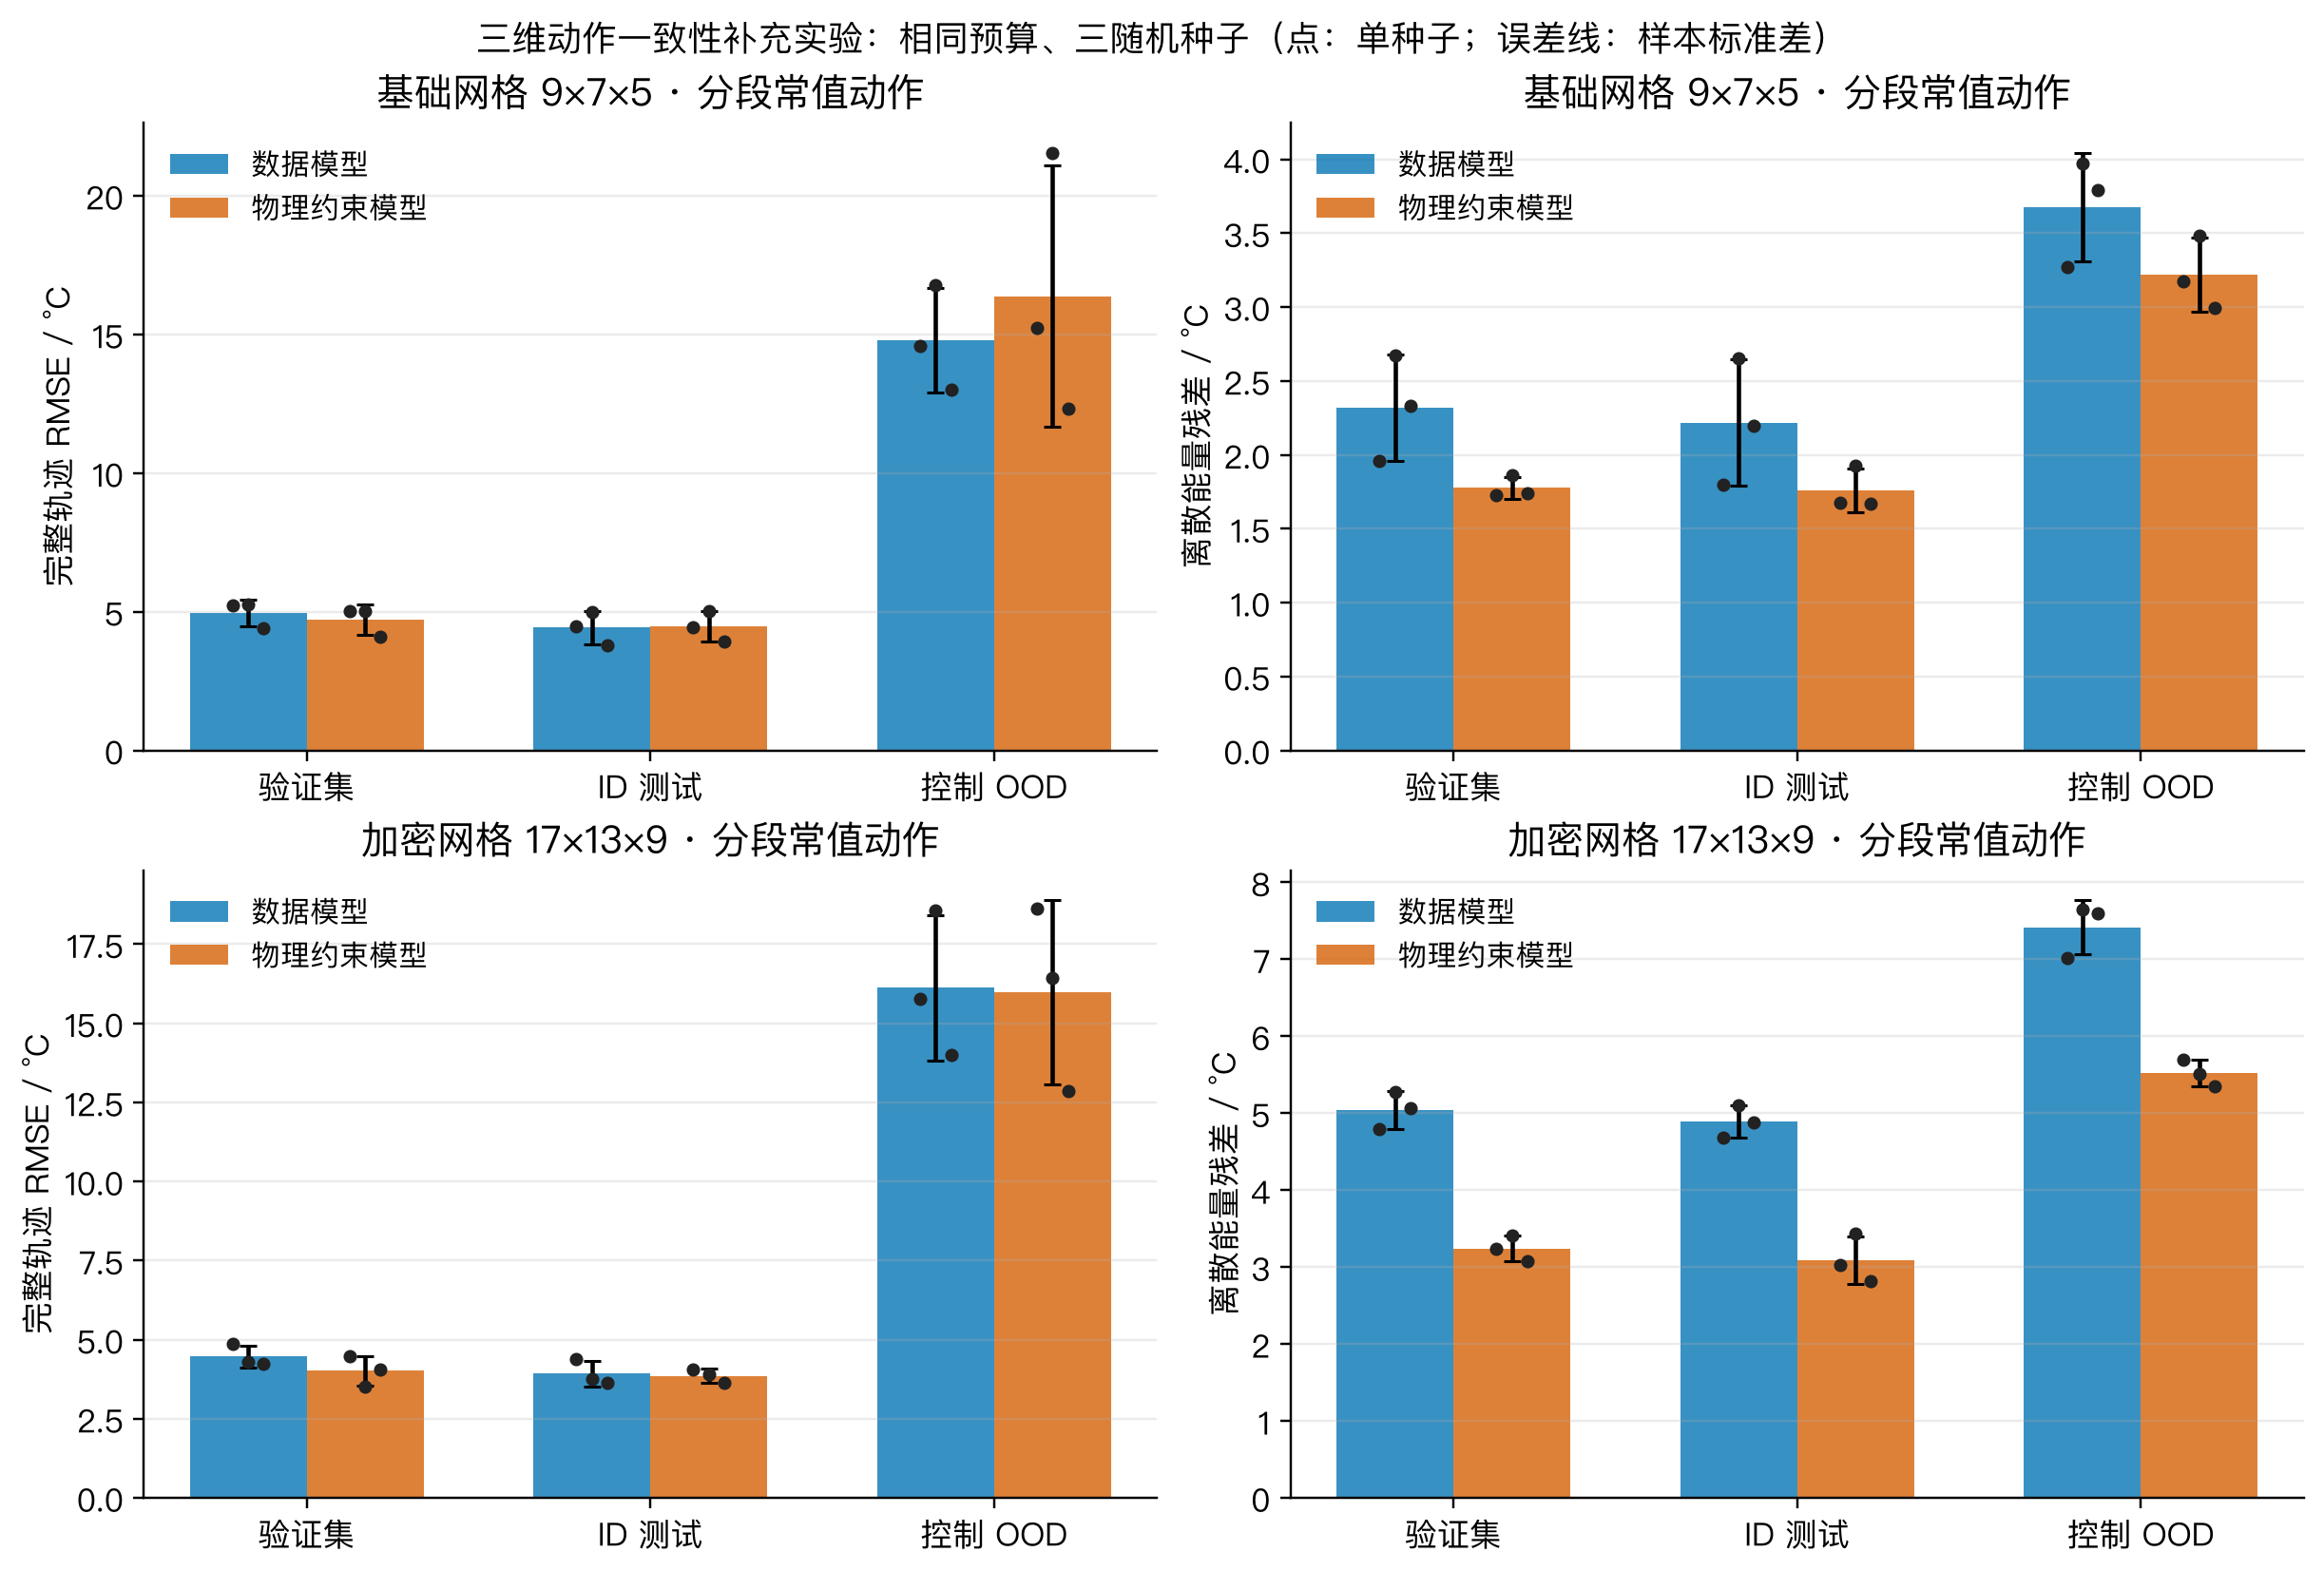
\includegraphics[width=0.98\textwidth]{three_dimensional_zoh_comparison.png}
  \caption{分段常值动作下，两种三维网格的滚动误差与离散能量残差；点表示单种子结果，误差线为样本标准差}
  \label{fig:three_dimensional_replicates}
\end{figure}

\subsect{固定工况的空间温度分布}

图\ref{fig:three_dimensional_cutaway}展示固定ID工况74、$t=\SI{192}{\second}$ 和模型种子42的空间温度分布，以 $25\times19\times13$ 网格的分段常值动作BDF解作为细参考场。每个面板切去朝向观察者的一个八分体，使三个中心切面与外表面同时可见；四面板使用统一色标，学习模型在 $17\times13\times9$ 原生网格上显示，不作显示插值。工况与时刻的选取依据见附录。

将细网格BDF场投影到模型网格后，该时刻显式欧拉、数据模型和物理约束模型的场RMSE分别为 $0.27$、$6.40$ 和 \SI{3.23}{\degreeCelsius}。物理约束模型误差小于数据模型、大于数值基线。该图限于固定案例的空间误差，总体预测性能由全部轨迹统计评价，跨几何泛化仍未检验。相关端淬数字孪生研究关注三维温度场重建，本文评价给定炉温动作下的未来状态递推\cite{midaoui2026jominy}。

\begin{figure}[H]
  \centering
  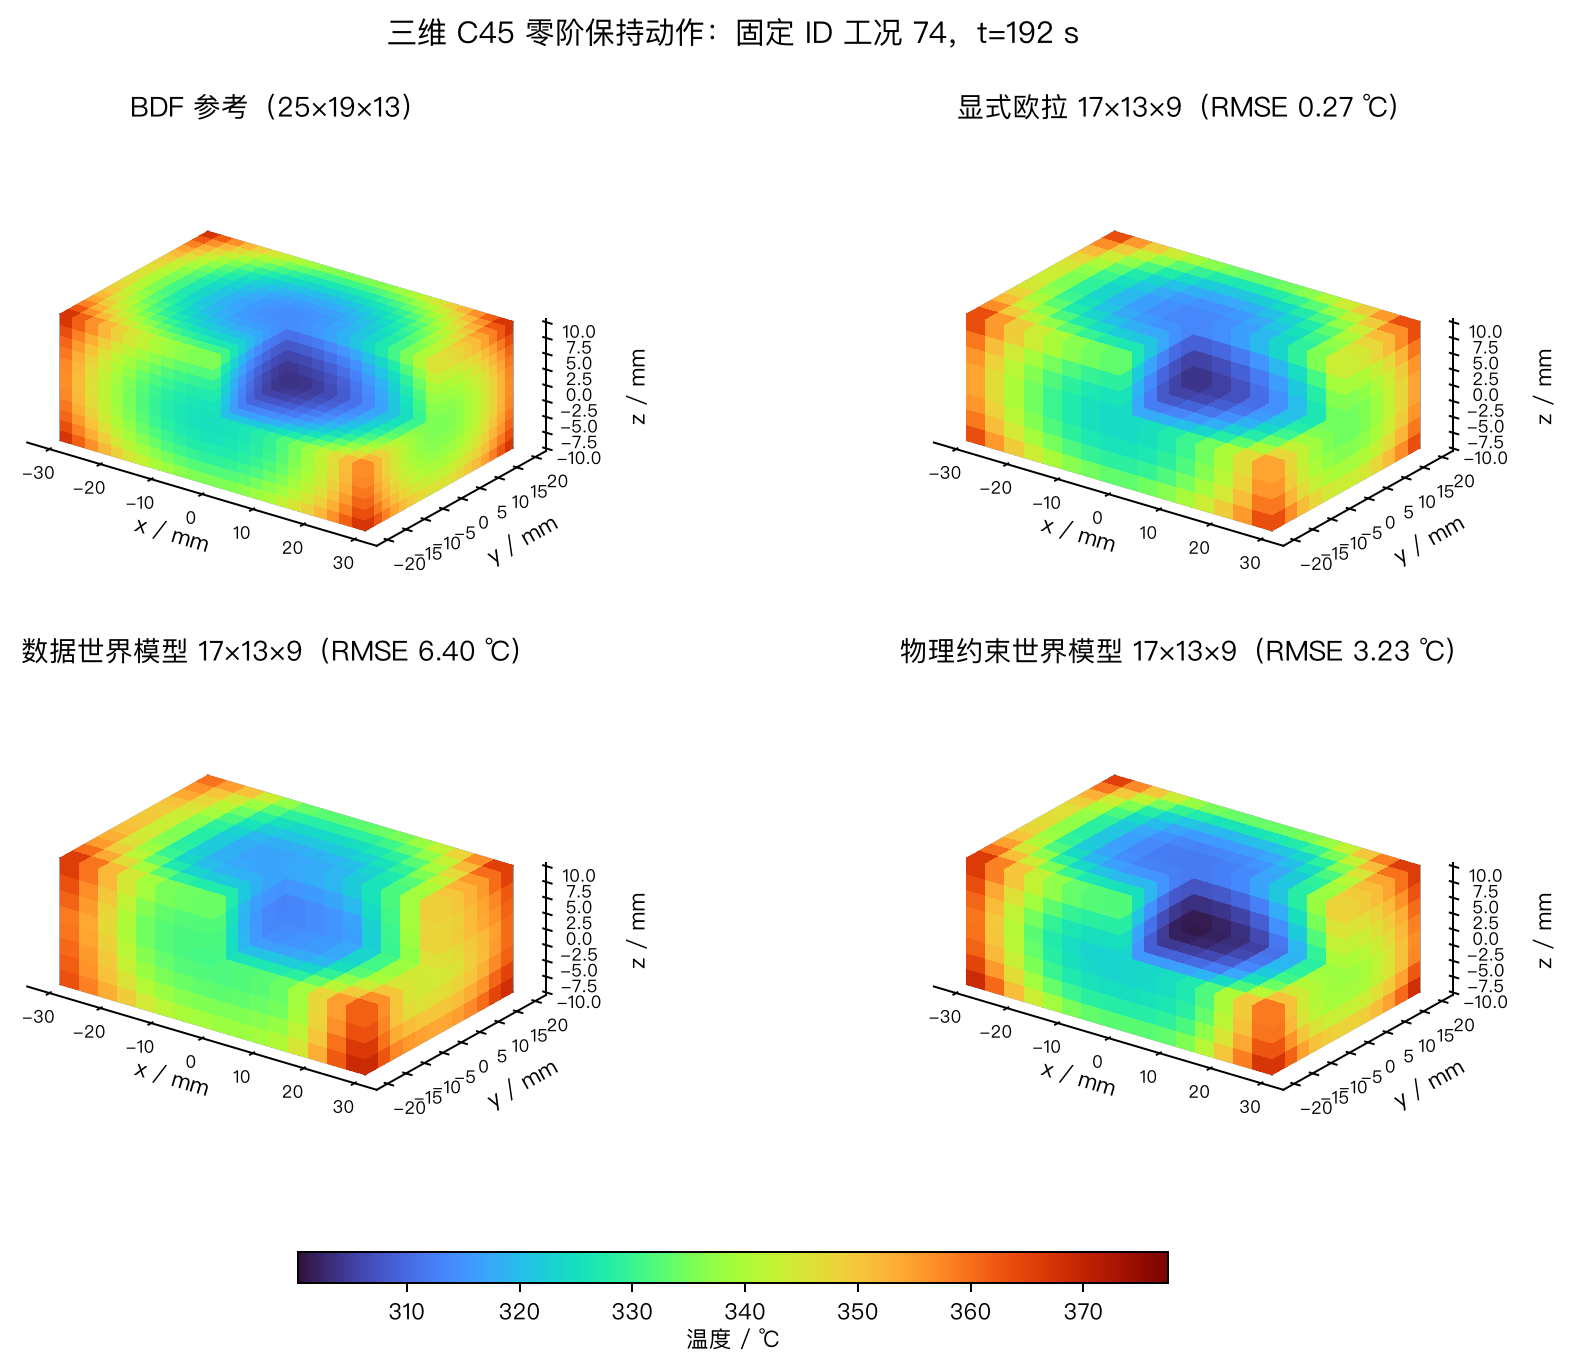
\includegraphics[width=0.95\textwidth]{three_dimensional_temperature_cutaway_zoh.png}
  \caption{分段常值炉温动作下，固定三维C45试块工况的八分体剖视温度场}
  \label{fig:three_dimensional_cutaway}
\end{figure}

物理约束改善了部分参数外推表现与离散一致性，控制曲线及三维 OOD 的稳定精度优势缺乏统计支持。自主 $\Heff$ 的预测收益限于已知动态边界及参考状态训练、验证条件；计时未建立相对低成本数值模型的综合优势。下一章评价有限测温条件下的状态与边界估计及其闭环控制表现。
